\documentclass[10pt]{beamer}
\usepackage[utf8]{inputenc}
\usepackage[T1]{fontenc}
\usepackage[spanish]{babel}
\usepackage{amsmath}
\usepackage{amssymb}
\usepackage{graphicx}
\usepackage{algorithm}
\usepackage{algpseudocode}
\usepackage{tikz}
\usepackage{booktabs}
\usepackage{xcolor}

% Configuración del tema
\usetheme{Madrid}
\usecolortheme{default}

% Colores personalizados
\definecolor{azulUni}{RGB}{0,102,204}
\definecolor{grisOscuro}{RGB}{64,64,64}
\definecolor{verdeClaro}{RGB}{46,125,50}

\setbeamercolor{structure}{fg=azulUni}
\setbeamercolor{palette primary}{bg=azulUni,fg=white}
\setbeamercolor{palette secondary}{bg=grisOscuro,fg=white}

% Información del documento
\title[Optimizadores de Gradiente]{Implementación de Técnicas de Descenso de Gradiente Estocástico y Variantes: Una Perspectiva desde el Análisis Numérico}
\subtitle{Una Comparación Experimental y Teórica}
\author[Trigueros]{Brandon Trigueros}
\institute[Universidad de Costa Rica]{Curso de Análisis Numérico\\Facultad de Ingeniería\\Universidad de Costa Rica}
\date{\today}

% Logo (opcional - descomenta si tienes logo)
%\logo{\includegraphics[height=0.8cm]{logo.png}}

\begin{document}

% Página de título
\begin{frame}
\titlepage
\end{frame}

% Índice
\begin{frame}{Índice}
\tableofcontents
\end{frame}

\section{Introducción}

\begin{frame}{¿Por qué importa el Descenso de Gradiente?}
\begin{alertblock}{¡Está en TODAS partes!}
\begin{itemize}
\item \textbf{Google}: PageRank optimiza rankings de páginas web
\item \textbf{Netflix}: Sistemas de recomendación personalizados  
\item \textbf{Tesla}: Conducción autónoma y visión computacional
\item \textbf{ChatGPT}: Entrenamiento de modelos de lenguaje masivos
\item \textbf{Medicina}: Diagnóstico por imágenes médicas (rayos X, resonancias)
\end{itemize}
\end{alertblock}

\begin{block}{El Desafío}
\begin{itemize}
\item \textbf{Problema}: Optimizar funciones con millones/billones de parámetros
\item \textbf{Datasets}: Terabytes de información (Twitter, YouTube, Amazon)
\item \textbf{Tiempo}: Entrenar GPT-3 costó \$4.6 millones en cómputo
\end{itemize}
\end{block}

\vspace{0.3cm}
\textcolor{azulUni}{\textbf{Pregunta clave:}} ¿Cómo hacer que estos algoritmos sean MÁS RÁPIDOS y EFICIENTES?
\end{frame}

\begin{frame}{La Analogía del Montañista}
\begin{columns}
\begin{column}{0.5\textwidth}
\begin{center}
\begin{tikzpicture}[scale=0.6]
% Dibujar la función de costo (paisaje montañoso) - más compacta
\draw[thick, blue, domain=-2.5:2.5, smooth, samples=80] 
    plot (\x, {0.4*(\x)^2 + 0.2*sin(2*\x r) + 1});

% Ejes coordenados - más pequeños
\draw[->] (-2.8,0.5) -- (2.8,0.5) node[right] {\tiny $\theta$};
\draw[->] (0,0.3) -- (0,2.5) node[above] {\tiny $J(\theta)$};

% Gradiente (flecha de pendiente) - más corta
\draw[->, thick, orange, line width=1.5pt] 
    (-1.5, {0.4*(-1.5)^2 + 0.2*sin(2*(-1.5) r) + 1}) -- 
    (-1, {0.4*(-1.5)^2 + 0.2*sin(2*(-1.5) r) + 1 - 0.4}) 
    node[midway, above, sloped, font=\tiny] {gradiente};

% Mínimo global (valle)
\filldraw[green!70!black] (0, 1) circle (2pt);
\node[green!70!black, below, font=\tiny] at (0, 0.8) {Valle};

% Trayectoria de descenso (línea punteada)
\draw[dashed, red, thick, line width=1pt] 
    (-1.5, {0.4*(-1.5)^2 + 0.2*sin(2*(-1.5) r) + 1}) -- 
    (-1, {0.4*(-1)^2 + 0.2*sin(2*(-1) r) + 1}) --
    (-0.5, {0.4*(-0.5)^2 + 0.2*sin(2*(-0.5) r) + 1}) --
    (0, 1);

% Niebla (área sombreada) - más compacta
\fill[gray!20, opacity=0.7] 
    (-2, 0.8) rectangle (-1, 2.2);
\node[gray!60, font=\tiny] at (-1.5, 2) {Niebla};

\end{tikzpicture}
\end{center}
\end{column}
\begin{column}{0.5\textwidth}
\textbf{Montañista perdido en la niebla:}
\begin{itemize}
\item Solo ve el \textcolor{red}{\textbf{terreno local}}
\item Quiere llegar al \textcolor{verdeClaro}{\textbf{valle más bajo}}
\item Estrategia: seguir la \textcolor{orange}{\textbf{pendiente más empinada}}
\end{itemize}

\vspace{0.3cm}
\textbf{En Machine Learning:}
\begin{itemize}
\item \textbf{Montaña} = función de error
\item \textbf{Posición} = parámetros
\item \textbf{Pendiente} = gradiente
\item \textbf{Valle} = mejor solución
\end{itemize}
\end{column}
\end{columns}
\end{frame}

\begin{frame}{Objetivos del Trabajo}
\begin{block}{Objetivo Principal}
Comparar experimentalmente cuatro técnicas de optimización:
\begin{itemize}
\item SGD básico
\item SGD con Momentum  
\item RMSProp
\item Adam
\end{itemize}
\end{block}

\begin{block}{Metodología}
\begin{itemize}
\item Implementación en Python desde cero
\item Experimento con regresión logística en dataset Iris
\item Análisis de curvas de convergencia
\end{itemize}
\end{block}

\begin{block}{Conexión con Análisis Numérico}
\begin{itemize}
\item Comparación con métodos de segundo orden
\item Análisis de convergencia y trade-offs computacionales
\end{itemize}
\end{block}
\end{frame}

\section{Fundamentos Teóricos}

\begin{frame}{Descenso de Gradiente Clásico}
\begin{block}{Fórmula Básica}
$$\boldsymbol{\theta}_{t+1} = \boldsymbol{\theta}_t - \eta \nabla_{\boldsymbol{\theta}} J(\boldsymbol{\theta}_t)$$
\end{block}

\begin{columns}
\begin{column}{0.5\textwidth}
\textbf{Ventajas:}
\begin{itemize}
\item Convergencia estable
\item Garantiza llegar al mínimo (funciones convexas)
\end{itemize}
\end{column}
\begin{column}{0.5\textwidth}
\textbf{Desventajas:}
\begin{itemize}
\item Muy lento con datasets grandes
\item Calcula gradiente completo en cada paso
\end{itemize}
\end{column}
\end{columns}

\vspace{0.5cm}
Donde: $\eta$ = tasa de aprendizaje, $J(\boldsymbol{\theta})$ = función de costo
\end{frame}

\begin{frame}{SGD: Descenso de Gradiente Estocástico}
\begin{block}{Idea Principal}
Usar solo \textbf{una muestra} (o pequeño mini-lote) por iteración:
$$\boldsymbol{\theta}_{t+1} = \boldsymbol{\theta}_t - \eta \nabla_{\boldsymbol{\theta}} \ell(\boldsymbol{\theta}_t; \mathbf{x}_{i(t)}, y_{i(t)})$$
\end{block}

\begin{alertblock}{Trade-off Fundamental}
\begin{itemize}
\item \textcolor{verdeClaro}{\textbf{+}} Mucho más rápido computacionalmente
\item \textcolor{verdeClaro}{\textbf{+}} Permite manejar datasets enormes
\item \textcolor{red}{\textbf{-}} Introduce ruido en las actualizaciones
\item \textcolor{red}{\textbf{-}} Trayectoria más errática
\end{itemize}
\end{alertblock}
\end{frame}

\begin{frame}{SGD con Momentum}
\begin{block}{Analogía Física}
Como una bola rodando que \textbf{acumula velocidad} y mantiene inercia
\end{block}

\begin{block}{Fórmulas}
\begin{align}
\mathbf{v}_t &= \gamma \mathbf{v}_{t-1} + \eta \nabla J(\boldsymbol{\theta}_t) \\
\boldsymbol{\theta}_{t+1} &= \boldsymbol{\theta}_t - \mathbf{v}_t
\end{align}
\end{block}

\begin{columns}
\begin{column}{0.5\textwidth}
\textbf{Beneficios:}
\begin{itemize}
\item Acelera en direcciones consistentes
\item Amortigua oscilaciones
\end{itemize}
\end{column}
\begin{column}{0.5\textwidth}
\textbf{Riesgo:}
\begin{itemize}
\item Puede "pasar de largo" el mínimo
\item Requiere ajuste cuidadoso de $\eta$
\end{itemize}
\end{column}
\end{columns}

\vspace{0.3cm}
Típicamente: $\gamma = 0.9$ (retiene 90\% de la velocidad previa)
\end{frame}

\begin{frame}{RMSProp}
\begin{block}{Problema que Resuelve}
Diferentes parámetros pueden necesitar diferentes tasas de aprendizaje
\end{block}

\begin{block}{Fórmulas}
\begin{align}
E[g_j^2]_t &= \rho E[g_j^2]_{t-1} + (1-\rho) g_{j,t}^2 \\
\theta_{j,t+1} &= \theta_{j,t} - \frac{\eta}{\sqrt{E[g_j^2]_t + \varepsilon}} g_{j,t}
\end{align}
\end{block}

\begin{exampleblock}{Intuición}
\begin{itemize}
\item Si un parámetro tiene gradientes grandes $\Rightarrow$ paso más pequeño
\item Si un parámetro tiene gradientes pequeños $\Rightarrow$ paso más grande
\item \textbf{Adaptación automática} por coordenada
\end{itemize}
\end{exampleblock}

Típicamente: $\rho = 0.9$, $\varepsilon = 10^{-8}$
\end{frame}

\begin{frame}{Adam: Lo Mejor de Dos Mundos}
\begin{block}{Combinación Inteligente}
Adam = Momentum + RMSProp
\end{block}

\begin{block}{Fórmulas (simplificadas)}
\begin{align}
m_{j,t} &= \beta_1 m_{j,t-1} + (1-\beta_1) g_{j,t} \quad \text{(momentum)} \\
v_{j,t} &= \beta_2 v_{j,t-1} + (1-\beta_2) g_{j,t}^2 \quad \text{(normalización)} \\
\theta_{j,t+1} &= \theta_{j,t} - \frac{\eta}{\sqrt{\hat{v}_{j,t}} + \varepsilon} \hat{m}_{j,t}
\end{align}
\end{block}

\begin{block}{¿Por qué es Popular?}
\begin{itemize}
\item Funciona bien "out-of-the-box"
\item Pocos hiperparámetros que ajustar
\item Robusto en muchos problemas
\end{itemize}
\end{block}

Valores por defecto: $\beta_1 = 0.9$, $\beta_2 = 0.999$, $\eta = 0.001$
\end{frame}

\section{Implementación del Experimento}

\begin{frame}{Diseño Experimental}
\begin{block}{Dataset Iris}
\begin{itemize}
\item 150 muestras de flores Iris
\item 4 características: longitud/ancho sépalos y pétalos
\item \textbf{Clasificación binaria}: Versicolor vs. Virginia
\item División: 80\% entrenamiento, 20\% prueba
\end{itemize}
\end{block}

\begin{block}{Modelo: Regresión Logística}
\begin{itemize}
\item Función sigmoide: $h_{\mathbf{w}}(\mathbf{x}) = \frac{1}{1 + e^{-\mathbf{w}^T\mathbf{x}}}$
\item Función de costo: Entropía cruzada binaria
\item Gradiente analítico: $\nabla J = \frac{1}{N}\sum_i (h(\mathbf{x}_i) - y_i)\mathbf{x}_i$
\end{itemize}
\end{block}
\end{frame}

\begin{frame}[fragile]{Implementación en Python}
\begin{block}{SGD Básico}
\begin{verbatim}
for epoch in range(epochs):
    for i in range(N):
        y_pred = sigmoid(np.dot(w, X[i]))
        grad = (y_pred - y[i]) * X[i]
        w = w - lr * grad
\end{verbatim}
\end{block}

\begin{block}{SGD con Momentum}
\begin{verbatim}
v = np.zeros(d)  # velocidad inicial
for epoch in range(epochs):
    for i in range(N):
        grad = compute_gradient(w, X[i], y[i])
        v = gamma * v + lr * grad
        w = w - v
\end{verbatim}
\end{block}
\end{frame}

\begin{frame}{Configuración de Hiperparámetros}
Después de experimentación, se eligieron:

\begin{table}[ht]
\centering
\begin{tabular}{lcc}
\toprule
\textbf{Algoritmo} & \textbf{Tasa de Aprendizaje} & \textbf{Parámetros Adicionales} \\
\midrule
SGD & 0.05 & - \\
SGD + Momentum & 0.03 & $\gamma = 0.9$ \\
RMSProp & 0.05 & $\rho = 0.9$, $\varepsilon = 10^{-8}$ \\
Adam & 0.05 & $\beta_1 = 0.9$, $\beta_2 = 0.999$ \\
\bottomrule
\end{tabular}
\end{table}

\begin{alertblock}{Nota Importante}
Momentum requirió menor tasa de aprendizaje para evitar inestabilidad
\end{alertblock}
\end{frame}

\section{Conexión con Análisis Numérico}

\begin{frame}{Método de Newton-Raphson vs. Descenso de Gradiente}
\begin{block}{Newton-Raphson (Segundo Orden)}
$$\boldsymbol{\theta}_{t+1} = \boldsymbol{\theta}_t - \mathbf{H}^{-1}(\boldsymbol{\theta}_t) \nabla J(\boldsymbol{\theta}_t)$$
donde $\mathbf{H}$ es la matriz Hessiana (segundas derivadas)
\end{block}

\begin{block}{Descenso de Gradiente (Primer Orden)}
$$\boldsymbol{\theta}_{t+1} = \boldsymbol{\theta}_t - \eta \nabla J(\boldsymbol{\theta}_t)$$
\end{block}

\begin{columns}
\begin{column}{0.5\textwidth}
\textbf{Newton-Raphson:}
\begin{itemize}
\item \textcolor{verdeClaro}{Convergencia cuadrática}
\item \textcolor{verdeClaro}{Pocas iteraciones}
\item \textcolor{red}{$O(n^3)$ por iteración}
\item \textcolor{red}{Hessiana puede no ser positiva definida}
\end{itemize}
\end{column}
\begin{column}{0.5\textwidth}
\textbf{Descenso de Gradiente:}
\begin{itemize}
\item \textcolor{red}{Convergencia lineal}
\item \textcolor{red}{Más iteraciones}
\item \textcolor{verdeClaro}{$O(n)$ por iteración}
\item \textcolor{verdeClaro}{Siempre estable}
\end{itemize}
\end{column}
\end{columns}
\end{frame}

\begin{frame}{¿Por qué no usar siempre Newton-Raphson?}
\begin{alertblock}{El Problema de Escalabilidad}
Para un modelo con $n$ parámetros:
\begin{itemize}
\item \textbf{Gradiente}: vector de tamaño $n$ → $O(n)$ memoria
\item \textbf{Hessiana}: matriz de tamaño $n \times n$ → $O(n^2)$ memoria
\item \textbf{Inversión}: $O(n^3)$ operaciones
\end{itemize}
\end{alertblock}

\begin{exampleblock}{Ejemplo Real: GPT-3}
\begin{itemize}
\item \textbf{Parámetros}: 175 mil millones ($n = 1.75 \times 10^{11}$)
\item \textbf{Hessiana}: $(1.75 \times 10^{11})^2 = 3 \times 10^{22}$ elementos
\item \textbf{Memoria}: $\sim 10^{14}$ TB (¡imposible!)
\end{itemize}
\end{exampleblock}

\vspace{0.3cm}
\textbf{Conclusión}: Necesitamos métodos de primer orden escalables → \textcolor{azulUni}{Descenso de Gradiente}
\end{frame}

\begin{frame}{Métodos Quasi-Newton: El Punto Intermedio}
\begin{block}{Idea Principal}
Aproximar la inversa de la Hessiana sin calcularla explícitamente
\end{block}

\begin{columns}
\begin{column}{0.5\textwidth}
\textbf{Métodos Quasi-Newton:}
\begin{itemize}
\item BFGS, L-BFGS
\item Aproximan $\mathbf{H}^{-1}$ iterativamente
\item Convergencia superlineal
\item $O(n^2)$ memoria
\end{itemize}
\end{column}
\begin{column}{0.5\textwidth}
\textbf{Métodos Adaptativos:}
\begin{itemize}
\item Adam, RMSProp
\item Aproximan información de segundo orden
\item Escalables a problemas masivos
\item $O(n)$ memoria
\end{itemize}
\end{column}
\end{columns}

\begin{alertblock}{Conexión Clave}
\textbf{Adam} puede verse como una aproximación diagonal de métodos Quasi-Newton:
$$\text{Adam} \approx \boldsymbol{\theta}_{t+1} = \boldsymbol{\theta}_t - \text{diag}(\mathbf{H}^{-1}) \nabla J(\boldsymbol{\theta}_t)$$
\end{alertblock}
\end{frame}

\section{Resultados y Análisis}

\begin{frame}{Curvas de Convergencia}
\begin{center}
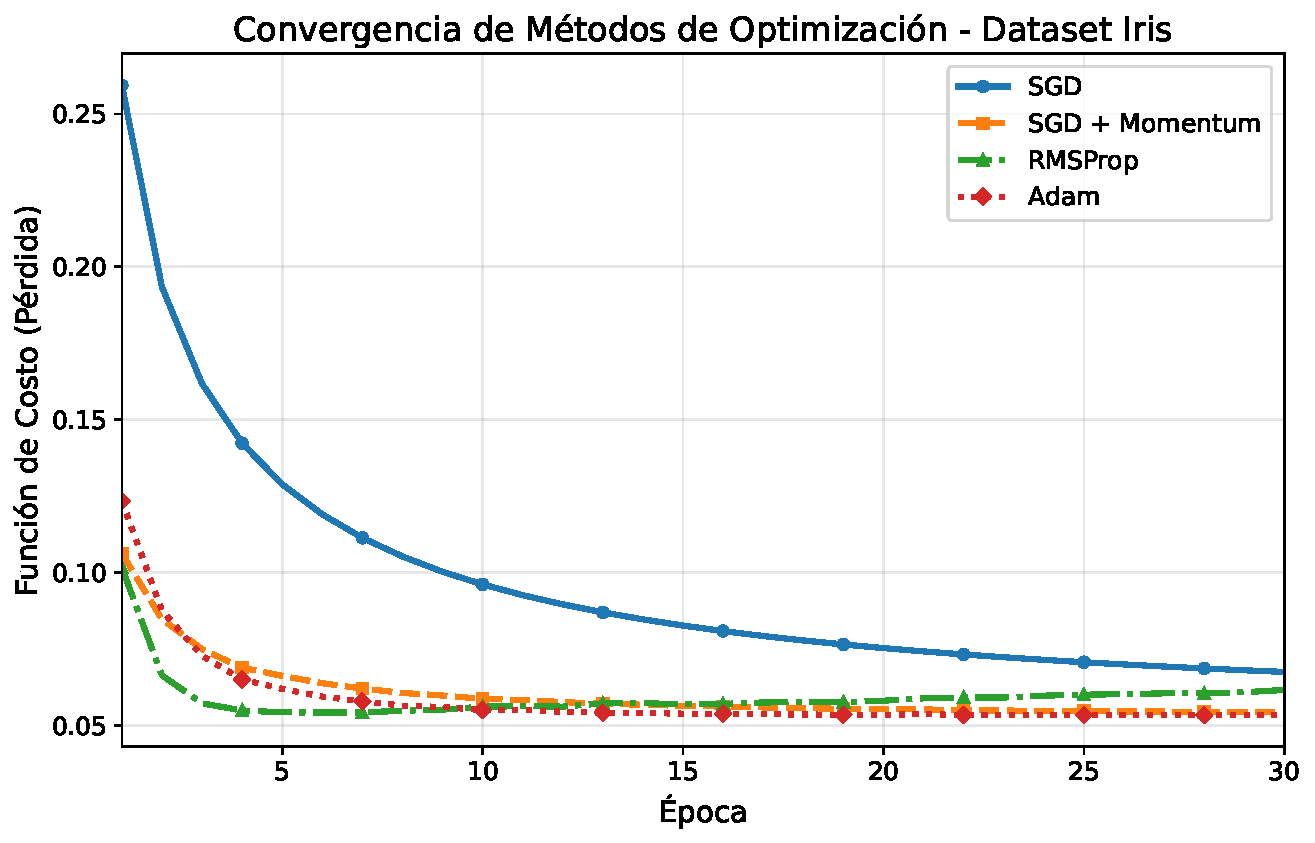
\includegraphics[width=0.85\textwidth]{curvas_convergencia.pdf}
\end{center}

\begin{itemize}
\item \textbf{Adam}: Convergencia más rápida (~5 épocas)
\item \textbf{RMSProp}: Buena velocidad, algo oscilante
\item \textbf{Momentum}: Descenso inicial rápido pero inestable
\item \textbf{SGD}: Más lento pero eventualmente converge
\end{itemize}
\end{frame}

\begin{frame}{Análisis Detallado de Resultados}
\begin{block}{Adam - El Ganador}
\begin{itemize}
\item Pérdida final: $\sim 0.12$ en solo 10 épocas
\item Curva suave y estable
\item Mínima necesidad de ajuste manual
\end{itemize}
\end{block}

\begin{block}{Momentum - Doble Filo}
\begin{itemize}
\item Descenso inicial más drástico (época 2: pérdida $\sim 0.1$)
\item \textcolor{red}{Pero oscilaciones significativas después}
\item Evidencia del problema de "sobrepaso"
\end{itemize}
\end{block}

\begin{block}{RMSProp vs SGD}
\begin{itemize}
\item RMSProp: Convergencia acelerada ($\sim 0.15$ final)
\item SGD: Lento pero confiable ($\sim 0.30$ a época 30)
\end{itemize}
\end{block}
\end{frame}

\begin{frame}{Métricas de Rendimiento Final}
\begin{table}[ht]
\centering
\small
\begin{tabular}{lccc}
\toprule
\textbf{Algoritmo} & \textbf{Costo Final} & \textbf{Precisión Train} & \textbf{Precisión Test} \\
\midrule
SGD & 0.067 & 96.25\% & 95.00\% \\
SGD + Momentum & 0.054 & 96.25\% & 95.00\% \\
RMSProp & 0.062 & 96.25\% & 90.00\% \\
Adam & 0.053 & 97.50\% & 95.00\% \\
\bottomrule
\end{tabular}
\end{table}

\begin{block}{Observaciones Importantes}
\begin{itemize}
\item Precisión final similar en todos los métodos
\item Diferencias principales en \textbf{velocidad de convergencia}
\item Adam ligeramente superior en precisión de entrenamiento
\end{itemize}
\end{block}
\end{frame}

\begin{frame}{Ventajas y Desventajas por Método}
\begin{columns}
\begin{column}{0.5\textwidth}
\begin{block}{SGD}
\textcolor{verdeClaro}{\textbf{Pros:}}
\begin{itemize}
\item Simple de implementar
\item Estable y confiable
\item Buena generalización
\end{itemize}
\textcolor{red}{\textbf{Cons:}}
\begin{itemize}
\item Convergencia lenta
\item Sensible a tasa de aprendizaje
\end{itemize}
\end{block}

\begin{block}{Momentum}
\textcolor{verdeClaro}{\textbf{Pros:}}
\begin{itemize}
\item Acelera convergencia inicial
\item Supera valles estrechos
\end{itemize}
\textcolor{red}{\textbf{Cons:}}
\begin{itemize}
\item Puede oscilar mucho
\item Difícil de calibrar
\end{itemize}
\end{block}
\end{column}

\begin{column}{0.5\textwidth}
\begin{block}{RMSProp}
\textcolor{verdeClaro}{\textbf{Pros:}}
\begin{itemize}
\item Adaptación automática
\item Maneja bien gradientes dispersos
\end{itemize}
\textcolor{red}{\textbf{Cons:}}
\begin{itemize}
\item Algo más complejo
\item Requiere ajuste de $\rho$
\end{itemize}
\end{block}

\begin{block}{Adam}
\textcolor{verdeClaro}{\textbf{Pros:}}
\begin{itemize}
\item Mejor de ambos mundos
\item Funciona "out-of-the-box"
\item Robusto y rápido
\end{itemize}
\textcolor{red}{\textbf{Cons:}}
\begin{itemize}
\item Posible overfitting
\item Mínimos más "afilados"
\end{itemize}
\end{block}
\end{column}
\end{columns}
\end{frame}

\section{Conclusiones}

\begin{frame}{Perspectiva del Análisis Numérico}
\begin{block}{Compromiso Fundamental}
Velocidad de convergencia vs. Escalabilidad computacional
\end{block}

\begin{table}[ht]
\centering
\small
\begin{tabular}{lccc}
\toprule
\textbf{Método} & \textbf{Convergencia} & \textbf{Costo/Iter} & \textbf{Memoria} \\
\midrule
Newton-Raphson & Cuadrática & $O(n^3)$ & $O(n^2)$ \\
Quasi-Newton & Superlineal & $O(n^2)$ & $O(n^2)$ \\
Adam & Lineal & $O(n)$ & $O(n)$ \\
SGD & Lineal & $O(n)$ & $O(n)$ \\
\bottomrule
\end{tabular}
\end{table}

\begin{alertblock}{Insight Clave}
Los métodos adaptativos modernos (Adam, RMSProp) aproximan información de segundo orden con costo de primer orden
\end{alertblock}
\end{frame}

\begin{frame}{Conclusiones Principales}
\begin{enumerate}
\item \textbf{Adam es el claro ganador} para convergencia rápida y facilidad de uso
\item \textbf{Momentum acelera} pero requiere cuidado en la calibración
\item \textbf{RMSProp} ofrece buen compromiso entre velocidad y estabilidad
\item \textbf{SGD básico} sigue siendo válido para casos que priorizan generalización
\end{enumerate}

\begin{block}{Desde el Análisis Numérico}
Los métodos estudiados representan diferentes estrategias para incorporar información de curvatura (segundo orden) manteniendo la escalabilidad computacional
\end{block}

\begin{alertblock}{Recomendación Práctica}
\begin{itemize}
\item \textbf{Para empezar}: Adam con parámetros por defecto
\item \textbf{Para ajuste fino}: Considerar híbrido (Adam inicial + SGD final)
\item \textbf{Para datos grandes}: RMSProp o Adam
\item \textbf{Para mejor generalización}: SGD con momentum
\end{itemize}
\end{alertblock}
\end{frame}

\begin{frame}{El Futuro de la Optimización}
\begin{block}{Tendencias Actuales}
\begin{itemize}
\item \textbf{Métodos híbridos}: Combinando lo mejor de diferentes enfoques
\item \textbf{Optimización automática}: Learning rate schedules adaptativos
\item \textbf{Aproximaciones de segundo orden}: Métodos quasi-Newton escalables
\item \textbf{Optimización distribuida}: Para modelos masivos como GPT
\end{itemize}
\end{block}

\begin{exampleblock}{Aplicaciones Emergentes}
\begin{itemize}
\item \textbf{Federated Learning}: Optimización distribuida sin centralizar datos
\item \textbf{Neural Architecture Search}: Optimización de arquitecturas
\item \textbf{Meta-learning}: Aprender a optimizar
\end{itemize}
\end{exampleblock}

\vspace{0.5cm}
\textcolor{azulUni}{\textbf{Mensaje final:}} La optimización es el corazón de la IA moderna
\end{frame}

\begin{frame}{Mensajes Clave}
\begin{center}
\Large
\textbf{No existe un optimizador universal}
\end{center}

\vspace{0.5cm}

\begin{itemize}
\item La elección depende del problema específico
\item Adam es un excelente punto de partida
\item Siempre monitorear tanto entrenamiento como validación
\item La implementación correcta es tan importante como la elección del algoritmo
\end{itemize}

\vspace{0.5cm}

\begin{center}
\textcolor{azulUni}{\textbf{El entendimiento teórico guía las decisiones prácticas}}
\end{center}
\end{frame}

\begin{frame}[plain]
\begin{center}
{\Huge \textbf{¿Preguntas?}}

\vspace{1.5cm}

{\Large Gracias por su atención}

\vspace{1cm}

\begin{columns}
\begin{column}{0.5\textwidth}
\centering
Brandon Trigueros\\
\texttt{brandon.trigueros@ucr.ac.cr}
\end{column}
\end{columns}

\vspace{1cm}

{\small Código disponible en: \texttt{https://github.com/BrandonTrigueros/gradient-descent-research}}
\end{center}
\end{frame}

% Página de agradecimiento
\begin{frame}
\begin{center}
\Large \textbf{¡Gracias por su atención!}

\vspace{1cm}

\textcolor{azulUni}{\huge \textbf{¿Preguntas?}}

\vspace{1cm}

\begin{tikzpicture}[scale=0.6]
% Función de costo optimizada
\draw[thick, blue, domain=-2:2, smooth] plot (\x, {0.5*(\x)^2 + 0.5});
\draw[->] (-2.5,0) -- (2.5,0) node[right] {$\theta$};
\draw[->] (0,0) -- (0,3) node[above] {$J(\theta)$};

% Camino del algoritmo
\draw[->, thick, red, dashed] (-1.5,1.625) -- (-1,1) -- (-0.5,0.625) -- (0,0.5);
\filldraw[green] (0,0.5) circle (3pt) node[below] {\small Óptimo};
\filldraw[red] (-1.5,1.625) circle (2pt) node[above] {\small Inicio};

% Etiquetas
\node at (0,-0.5) {\small \textbf{Convergencia exitosa}};
\end{tikzpicture}

\vspace{0.5cm}

\textit{``En optimización, como en la vida, el camino más corto no siempre es el más eficiente''}

\end{center}
\end{frame}

% Diapositivas de respaldo (opcional)
\appendix

\begin{frame}{Respaldo: Fórmulas Detalladas de Adam}
\begin{block}{Algoritmo Completo}
\begin{align}
m_t &= \beta_1 m_{t-1} + (1-\beta_1) g_t \\
v_t &= \beta_2 v_{t-1} + (1-\beta_2) g_t^2 \\
\hat{m}_t &= \frac{m_t}{1-\beta_1^t} \quad \text{(corrección de sesgo)} \\
\hat{v}_t &= \frac{v_t}{1-\beta_2^t} \quad \text{(corrección de sesgo)} \\
\theta_{t+1} &= \theta_t - \frac{\eta}{\sqrt{\hat{v}_t} + \varepsilon} \hat{m}_t
\end{align}
\end{block}

\begin{itemize}
\item $m_t$: estimación del primer momento (media)
\item $v_t$: estimación del segundo momento (varianza no centrada)
\item Las correcciones de sesgo son importantes en las primeras iteraciones
\end{itemize}
\end{frame}

\begin{frame}{Respaldo: Datos del Experimento}
\begin{table}[ht]
\centering
\footnotesize
\begin{tabular}{c|cccc}
\toprule
\textbf{Época} & \textbf{SGD} & \textbf{Momentum} & \textbf{RMSProp} & \textbf{Adam} \\
\midrule
1 & 0.259 & 0.106 & 0.102 & 0.124 \\
2 & 0.193 & 0.085 & 0.067 & 0.088 \\
5 & 0.129 & 0.066 & 0.054 & 0.062 \\
10 & 0.099 & 0.058 & 0.055 & 0.054 \\
20 & 0.078 & 0.053 & 0.060 & 0.053 \\
30 & 0.068 & 0.054 & 0.062 & 0.053 \\
\bottomrule
\end{tabular}
\caption{Evolución del costo de entrenamiento}
\end{table}

\begin{itemize}
\item Adam converge más rápido en las primeras épocas
\item Momentum muestra la mayor reducción inicial pero luego oscila
\item SGD mejora de manera más gradual y consistente
\end{itemize}
\end{frame}

\end{document}
